\documentclass{article}
\usepackage{graphicx} % Required for inserting images
\usepackage{amsmath}
\usepackage{matlab-prettifier}
\usepackage{amssymb}

\title{Homework 2: \\ Chebyshev Polynomials \& FFT}
\author{Devin Smith \\ UIN: 330000494}
\date{Systems Analysis \\ AERO 666}


\begin{document}

\maketitle

\section{Project 1}
\subsection{Introduction}
In this problem, we will use Chebyshev polynomials of the second kind to solve ordinary differential equations. 
\par
Chebyshev polynomials of the second kind have the domain $[-1, 1]$, and are given by $U_0(x) = 1, U_1(x) = 2x$, together with the recursive relation $U_{n+1}(x)=2xU_n(x)-U_{n-1}(x)$. Furthermore, they are obtained as the derivatives of the Chebyshev polynomials of the first kind, that is to say that, $\frac{d}{dx}T_n(x)=nU_{n-1}(x)$.
\par
We are interested in evaluating the Chebyshev polynomials on special nodes that are approximated by $x_i=-cos(\frac{i\pi}{N+1})$, for some $i=1,...,N$. These can be verified to be the roots of the $U_n(x),n=N$. Let us now implement the following elements to write our own linear integration routine. We will integrate $\dot{y}=-\alpha y,y(t_0)=c$. If we want to integrate this equation
in the domain $t \in [0,t_f]$, we have to first convert this equation to change the domain to $x \in [-1, 1]$. This is accomplished by re-writing the differential equation as $\frac{dy}{dx}=y'=\dot{y}\frac{dt}{dx}=-\alpha(\frac{t_f}{2})y=-\alpha_1 y$.
\par
\subsection{Tasks}
Answer the following questions by implementing appropriate functions.
\begin{enumerate}
    \item Write a function to evaluate arbitrary number of Chebyshev polynomials (2nd kind) at a given (not necessarily the node 
    points). The inputs to this function are the number of Chebyshev polynomials you need (say $n$) and the vector of points (supplied as a row/column matrix) written as $\mathbf{x}$. So the output of this function for a given value of may be written by the row matrix $\mathbf{U}({x_1})^T= \begin{bmatrix}
        U_0(x_1) & U_1(x_1) & \dots & U_n(x_1)
    \end{bmatrix}$ $(1 \times (n+1)$ matrix)

    \item Write a separate function to take as an input $n$ (desired polynomial order) and output the roots of the Legendre polynomial $U_n(x)$ in the form of a column vector $\mathbf{x}=\begin{bmatrix}
        x_1 & x_2 & \dots & x_n
    \end{bmatrix}$. Note that this is an $n$ (column) vector.

    \item Now combine both results to evaluate the Chebyshev matrix, where each row corresponds to the Chebyshev polynomials evaluated at the roots of the $n$th polynomial. We should get a $n \times n+1$ matrix that looks like
    $
    \begin{bmatrix}
        U_0(x_1) & U_1(x_1) & \dots & U_n(x_1) \\
        U_0(x_2) & U_1(x_2) & \dots & U_n(x_2) \\
        \vdots & \vdots & \ddots & \vdots \\
        U_0(x_n) & U_1(x_n) & \dots & U_n(x_n) \\
    \end{bmatrix}.  
    $
    Investigate if the first $n$ columns are orthogonal to each other, and verify discrete orthogonality. What is the value of the last column, why do you think there is something strange about the last column evaluations?

    \item Now, let us try to construct the integration matrix based on these evaluations. Derive the identity $\int U_ndx = \frac{1}{2(n+1)}U_{n+1}-\frac{1}{2(n+1)}U_{n-1}$, with the first two integrals written as $\int U_0dx=x=\frac{1}{2}U_1$. The basis for this identity is the related recurrence definition of the Chebyshev polynomials $T_n(x)=\frac{1}{2}(U_n(x)-U_{n-2}(x))$, and the fact that the Chebyshev polynomials of the second kind are the derivatives of the Chebyshev polynomials of the first kind. $U_{n-1}=\frac{1}{n}\frac{dT_n}{dx}$. To prove $T_n(x)=\frac{1}{2}(U_n(x)-U_{n-2}(x))$, you will need the following 
    identities, $U_{n+1}=xU_n+T_{n+1}$, $T_{n+1}=xT_n-(1-x^2)U_{n-1}$, and the interesting identity that $T_m(x)U_n(x)=\frac{1}{2}(U_{n+m}(x)+U_{n-m}(x))$, when $n \geq m-1$. 
    \par
    We make use of the following (indefinite) integral identities, $\int U_ndx=\frac{1}{2n+2}(U_{n+1}-U_{n-1})$, $\forall n \geq2$, $\int U_0dx=\frac{1}{2}U_1$, $\int U_1dx=\frac{1}{4}(U_0+U_2)$. Therefore, one can evaluate the integrals of the Legendre polynomials by simply observing that 
    \begin{equation*}
    \int 
    \begin{bmatrix}
        U_0(x) & U_1(x) & \dots & U_n(x)
    \end{bmatrix}dx = 
    \end{equation*}
    \begin{equation*}
    \begin{bmatrix}
        U_0(x) & U_1(x) & \dots & U_n(x)
    \end{bmatrix}
    \begin{bmatrix}
        0 & \frac{1}{4} & 0 & 0 & \dots & 0 & 0 \\
        1 & 0 & -\frac{1}{6} & 0 & \dots & 0 & 0 \\
        0 & \frac{1}{4} & 0 & -\frac{1}{8} & \dots & 0 & 0 \\
        0 & 0 & \frac{1}{6} & 0 & \dots & 0 & 0 \\
        \vdots & \vdots & \vdots & \vdots & \ddots & \vdots & \vdots \\
        0 & 0 & 0 & 0 & \dots & -\frac{1}{2n+2} & 0 \\
        0 & 0 & 0 & 0 & \dots & 0 & -\frac{1}{2n} \\
        0 & 0 & 0 & 0 & \dots & \frac{1}{2n+2} & 0 \\
    \end{bmatrix}
    \end{equation*}
    \begin{equation*}
        =UF
    \end{equation*}

    Note that the banded diagonal matrix $F$ on the right-hand side is a constant and does not depend on the functions. This is to say that we can evaluate the integrals of the Chebyshev polynomials for free (virtually) if we have the matrix $U$. We do have the matrix $U(x)$ evaluated at the Chebyshev nodes from item 3. Write a function to evaluate the matrix $F$ above.

    \item Let solution of the linear differential equation $\dot{y}=-\alpha y$ be written as a linear combination of the Chebyshev polynomials as $y(x)= \sum_{j=0}^{n-1} a_jU_j(x)$. Then the approximation formula in this equation can be written as $y(x_j)= \sum_{j=0}^{n-1} a_jU_j(x_j)$. In terms of the matrices we already populated, this is written as $\mathbf{y}=U(\mathbf{x})\mathbf{a}$. Here, the vector of unknown coefficients is written as the column matrix $\mathbf{a}$ and the solution evaluated at node point set $\mathbf{x}$ is given by $\mathbf{y}$. We then write the integral equation (we desire to solve) as $y(x_j) - y(-1)= -\alpha_1\sum_{j=0}^{n-1} \int_{-1}^{x_j}U_j(x_j)dx$. This equation can also be written as $\sum_{j=0}^{n-1} a_jU_j(x_j)-y(-1)= -\alpha_1\sum_{j=0}^{n-1} a_j(\int_{-1}^{x_j}U_j(x_j)dx)$. The solution of the differential equation can then be written as the linear system, $[U + \alpha_1(UF-\mathbf{o}\mathbf{U}(-1)F)]\mathbf{a}=y(-1)\mathbf{o}$, where the matrix $\mathbf{o} \in \mathbb{R}^{n-1\times 1}$ is a matrix of ones.
    \par
    Note that one can write the conditions from neighboring node points and not necessarily the integral from initial conditions to the current time step. Implement the above integration process.
    \par
    It is helpful to choose a small order for the Chebyshev polynomials (small - do not exceed 15 - 20) because the coefficient magnitudes can grow rapidly.

    \item Note that the true solution is given by $y(t)=y(0)e^{-\alpha (t-t_0)}=ce^{-\alpha (t-t_0)}$. Compare the errors incurred by the integration process developed in this problem.
\end{enumerate}

\subsection{Solution}
\begin{enumerate}
    \item This is the function to take n as an input and output the roots of the Chebyshev polynomial in the form of a column vector.
    \begin{lstlisting}[style=Matlab-editor]
function Uj = Chebyshev(xj, n)
    Uj = zeros(1, n + 1);
    Uj(1) = 1;
    if n >= 2
        Uj(2) = 2*xj;
    end
    if n > 2
        for i = 2: n
            Uj(i+1) = (2*xj*Uj(i) - Uj(i-1));
        end
    end
end
    \end{lstlisting}
 \item This is the function to take n as an input and output the roots of the Chebyshev polynomial in the form of a column vector.
 \begin{lstlisting}[style=Matlab-editor]
function x = ChebyshevRoot(n)
    x = zeros(n,1);
    for i = 1:n
        x(i) = -cos(i*pi/(n+1));
    end
end
    \end{lstlisting}
\item Combining the results of the previous two functions, this function creates the Chebyshev matrix. Additionally, this was used to investigate if the first $n$ columns are orthogonal and verify discrete orthogonality when using the Chebyshev roots. The the last column matrix was investigated as well when using the Chebyshev roots.
    \begin{lstlisting}[style=Matlab-editor]
function U = ChebyshevMatrix(n, x)
    U = zeros(length(x),n+1);
    for i = 1:length(x)
        U(i,:) = Chebyshev(x(i), n);
    end
end

function orthogonal = orthogonal(n, x, weighted)
    U = ChebyshevMatrix(n, x);

    if weighted
        for i = 1:n
            U(i,:) = U(i,:)*sqrt(1 - x(i)^2);
        end
    end

    sum = 0;
    for i = 1:n-1
        for j = (i+1):n
            dot = round(abs(U(:,i)'*U(:,j)),12);
            sum = sum + dot;
        end
    end
    
    if sum > 0
        orthogonal = false;
    else
        orthogonal = true;
    end
end
    \end{lstlisting}
    
\item The derivation of the identity mentioned Task 4 of Section 1.2 was attempted, however, while I was able to solve for the integral formula for $U_n$, I was unable to fully derive the identity for $T_n$ (see last page of report for work). A function was made to create the integration matrix.
    \begin{lstlisting}[style=Matlab-editor]
function F = FMatrix(n)
    F = zeros(n+1,n+1);
    for i = 1:n+1
        if i == 1
            F(i+1,i) = 1/2;
        elseif i == 2
            F(i-1,i) = 1/4;
            F(i+1,i) = 1/4;
        elseif i <= n
            F(i-1, i) = -1/(2*(i-1)+2);
            F(i+1, i) = 1/(2*(i-1)+2);
        else
            F(i-1, i) = -1/(2*(i-1));
        end
    end
end
    \end{lstlisting}

\item The previous functions were all used to implement the integration process in a single function. 

    \begin{lstlisting}[style=Matlab-editor]
function a = ChebyshevODE(n, x, alpha1, y0)
    U = ChebyshevMatrix(n, x);
    F = FMatrix(n);
    o = ones(length(x), 1);
  
    A = U + alpha1*(U*F - o*U(1,:)*F);
    b = y0*o;
    a = A \ b;
end
    \end{lstlisting}

\item Using all these functions, the analytical solution and the approximation using Chebyshev polynomials were evalutated and compared. 

\begin{lstlisting}[style=Matlab-editor]
% let dy/dt = y, y(0) = 1, 0 <= t <= 5
alpha = 2;
y0 = 5;
t = linspace(0,5,1000);

% chebyshev parameters
n = 10;                     % polynomial order
x = linspace(-1,1, 100)';   % x values to evaluate

% checking orthogonality (chebyshev roots)
Orth = orthogonal(n, ChebyshevRoot(n), 0);
discreteOrth = orthogonal(n, ChebyshevRoot(n), 1);

% mapping between x and t
alpha1 = alpha*t(end)/2;
x_map = (x - x(1))*t(end)/2 + t(1);

% solution in x
a = ChebyshevODE(n, x, alpha1, y0);
U = ChebyshevMatrix(n, x);
yApprox = U*a;
yTrue = y0*exp(-alpha1*(x-x(1)));
yError = yApprox - y0*exp(-alpha1*(x-x(1)));

% solution in t
yApprox_t = U*a;
yTrue_t = y0*exp(-alpha*(t-t(1)));
yError_t = yApprox - y0*exp(-alpha*(x_map-t(1)));
    \end{lstlisting}

\end{enumerate}

\subsection{Results}

In step 4, it was verified that the $U$ matrix is not orthogonal by itself, however, when weighting the rows via  $1-x_j^2$, it was found that the matrix was orthogonal. Additionally, it was found that the last column for the matrix is a zero column vector. The Chebyshev polyomials are constructed using the nodal points, and multiples of them. These nodal points are periodic in nature as they are constructed using a cosine. Because of this, the last column will always converge to zero. 
\par
For step 6, the Chebyshev Approximation is able to accurately match the anyltical solution for $y=5e^{-2t}$, $t \in [0, 5]$. In the Chebyshev approximation, the polynomial order used was $n=10$, and 100 $x$ values from -1 to 1 were used. The error between the solutions was on the order of $10^{-4}$.

\begin{figure}[h]
    \centering
    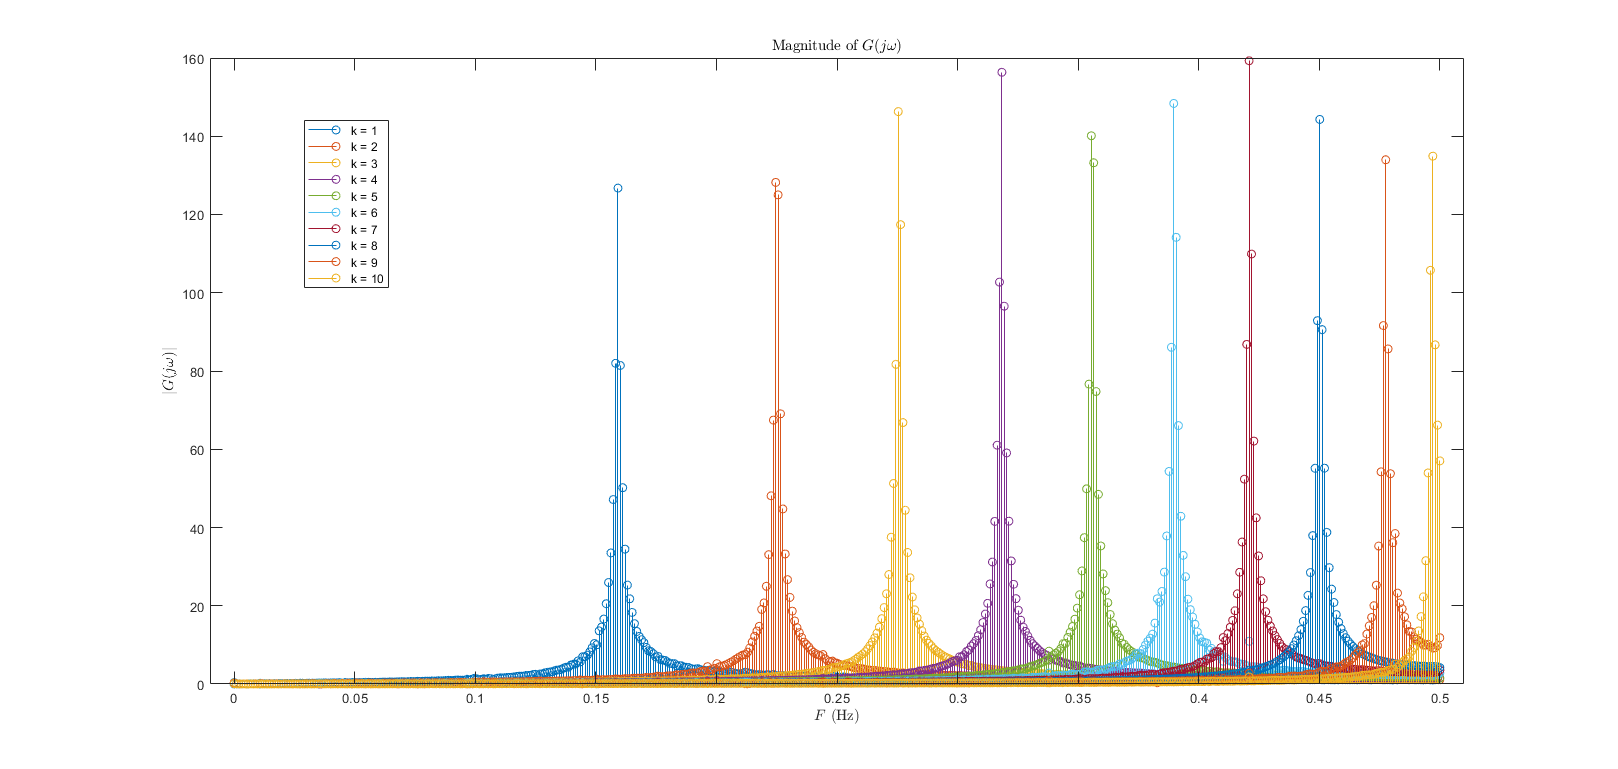
\includegraphics[width=.8\linewidth]{untitled.png}
    \caption{Approximate and Analytical Solution in $x$}
    \label{fig:enter-label}
\end{figure}

\begin{figure}[h]
    \centering
    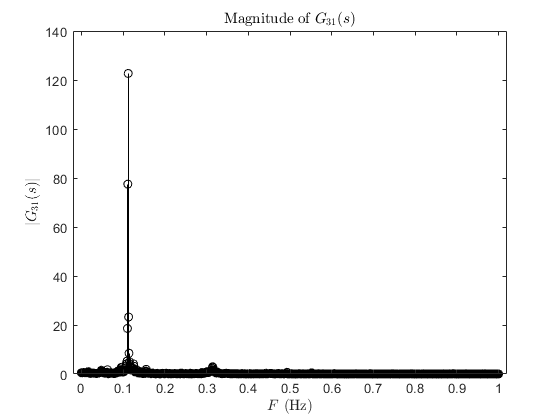
\includegraphics[width=.8\linewidth]{untitled2.png}
    \caption{Solution Error in $x$}
    \label{fig:enter-label}
\end{figure}

\begin{figure}[h]
    \centering
    \includegraphics[width=.8\linewidth]{untitled3.png}
    \caption{Approximate and Analytical Solution in $t$}
    \label{fig:enter-label}
\end{figure}

\begin{figure}[h]
    \centering
    \includegraphics[width=.8\linewidth]{untitled4.png}
    \caption{Solution Error in $t$}
    \label{fig:enter-label}
\end{figure}

\clearpage
\section{Project 2}
\subsection{Introduction}
This problem prepares you to compute the discrete Fourier transform using the FFT algorithm. Consider the signal $u(t) = cos(\omega_c t)$ with $\omega_c=3\pi$ rad.

\subsection{Tasks}
Follow the instructions to construct the Fourier transform from sampled data.

\begin{enumerate}
    \item Sample this true signal with a sampling frequency of Hz for a time period of 256 seconds. Let us call it y(1:Ns,1).
    \item Choose some parameters for the discrete Fourier transform (DFT), Np = 1024. Compute the discrete Fourier transformation (DFT) using the command: Ys = fft(y, Np)/Np; Frequency can be mapped as w = 0.5*fs*linspace(0 ,1,Np/2+1); This is frequency in Hz. Plot the magnitude of the signal. Write your observation about what you can say about the magnitude of the DFT. Plot the phase of the signal.
    \item Vary the frequency of the signal to and . Plot the DFT for the new signals. Explain what you see with respect to the ideal continuous Fourier transform you know from the theoretical results.
\end{enumerate}

\subsection{Solution}

\begin{enumerate}
    \item A function was created to sample the cosine function at a given set of time values and a given $\omega_c$ value.

        \begin{lstlisting}[style=Matlab-editor]
function u = y(t, coeff)
    u = cos(coeff*pi*t);
end

fs = 4;                 % frequency in Hz
T = 256;                % final time in s
t = 1/fs:1/fs:T;        % sampled time vals
Ns = T*fs;              % number of samples

    \end{lstlisting}
\item Code was written to compute the discrete Fourier transformation with Np = 1024. The magnitude and phase of the signal are plotted as well.
        \begin{lstlisting}[style=Matlab-editor]
Np = Ns;
w = 0.5*fs*linspace(0, 1, Np/2 + 1);

Ys = fft(y(t, 3),Np)/Np;
Ymag = abs(round(Ys(1:Np/2 + 1),10));
Yphase = angle(round(Ys(1:Np/2 + 1),10));
        
% plot data
figure;
omega = ['\omega_c = ' num2str(3) '\pi'];
subplot(2,1,1); plot(w,Ymag, "k");
title(omega);
xlabel('\omega (Hz)'); ylabel('Magnitude'); 
grid on;
subplot(2,1,2); plot(w,Yphase, "k");
xlabel('\omega (Hz)'); ylabel('Phase (rad)'); 
grid on;
        \end{lstlisting}

\item Code was written to repeat the process but for varying $\omega_c$ from $1\pi$ to $5\pi$. The plots can be combined together or plotted separately, and the interval which $\omega_c$ is incremented is changeable as well. 

        \begin{lstlisting}[style=Matlab-editor]
fstep = 0.25;   % step size for varying w_c
combined = 1;   % plot together or separately

if combined
    figure;
    for i = 1:fstep:5
        % fft
        Ys = fft(y(t, i),Np)/Np;
        Ymag = abs(round(Ys(1:Np/2 + 1),10));
        Yphase = angle(round(Ys(1:Np/2 + 1),10));
        
        % get text placement
        mag_text = max(Ymag) + max(Ymag)*.1;
        phase_text = max(Yphase) + max(Yphase)*.1;
        omega_text = w(find(Ymag==max(Ymag)));
        if phase_text == 0
            phase_text = 0.3;
        end
        if i > 4 && i < 8
            mag_text = mag_text + 0.1;
            phase_text = phase_text + 0.3;
        end
        
        % plot data and text
        omega = ['\omega_c = ' num2str(i) '\pi'];
        subplot(2,1,1); plot(w,Ymag, 'k', DisplayName=omega); hold on;
        xlim([0 2.1]); ylim([0 1.3])
        text(omega_text, mag_text, omega, HorizontalAlignment='center')
        xlabel('\omega (Hz)'); ylabel('Magnitude'); grid on;
        subplot(2,1,2); plot(w,Yphase, 'k', DisplayName=omega); hold on;
        text(omega_text, phase_text, omega, HorizontalAlignment='center')
        xlim([0 2.1]); ylim([0 4]);
        xlabel('\omega (Hz)'); ylabel('Phase (rad)'); grid on;
    end
else
    for i = 1:fstep:5
        % fft
        Ys = fft(y(t, i),Np)/Np;
        Ymag = abs(round(Ys(1:Np/2 + 1),10));
        Yphase = angle(round(Ys(1:Np/2 + 1),10));
        
        % plot data
        figure;
        omega = ['\omega_c = ' num2str(i) '\pi'];
        subplot(2,1,1); plot(w,Ymag);
        title(omega);
        xlabel('\omega (Hz)'); ylabel('Magnitude'); grid on;
        subplot(2,1,2); plot(w,Yphase);
        xlabel('\omega (Hz)'); ylabel('Phase (rad)'); grid on;
    end
end
        \end{lstlisting}

\end{enumerate}


\subsection{Results}

The DFT was created for $\omega_c$ from $1\pi$ to $5\pi$, and it was additionally checked up to $8\pi$.  As expected, the DFT plots show a single spike of magnitude and phase for a given $\omega_c$. It was found that until $\omega_c = 4\pi$, the amplitude of the signal was 0.5, and once $\omega_c = 4\pi$, the amplitude of the signal was 1 for multiples of $4\pi$. I theorize that this is related to the Nyquist frequency and Shannon's sampling theorem, and aliasing, as we are sampling the signal at 4 Hz. Furthermore, it can be seen that the phase of the signal increases as $\omega_c \rightarrow 4\pi$, and then decreases after.

\begin{figure}[h]
    \centering
    \includegraphics[width=.8\linewidth]{untitled5.png}
    \caption{DFT for $\omega_c = 3\pi$}
    \label{fig:enter-label}
\end{figure}

\begin{figure}[h]
    \centering
    \includegraphics[width=0.8\linewidth]{untitled8.png}
    \caption{DFT for $\omega_c$ = $1\pi$ to $5\pi$, step size = $1\pi$}
    \label{fig:enter-label}
\end{figure}

\begin{figure}[h]
    \centering
    \includegraphics[width=0.8\linewidth]{untitled7.png}
    \caption{DFT for $\omega_c$ = $1\pi$ to $5\pi$, step size = $0.5\pi$}
    \label{fig:enter-label}
\end{figure}

\begin{figure}[h]
    \centering
    \includegraphics[width=1\linewidth]{untitled6.png}
    \caption{DFT for $\omega_c$ = $1\pi$ to $5\pi$, step size = $0.25\pi$}
    \label{fig:enter-label}
\end{figure}

\begin{figure}[h]
    \centering
    \includegraphics[width=1\linewidth]{untitled9.png}
    \caption{DFT for $\omega_c$ = $1\pi$ to $8\pi$, step size = $0.25\pi$}
    \label{fig:enter-label}
\end{figure}


\end{document}
